 \subsubsection{UC5 - Visualizzazione beni e servizi}
  \begin{figure}[H]
 	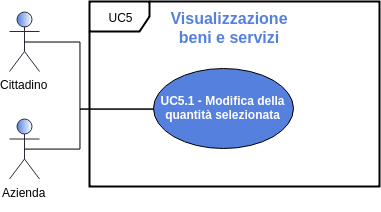
\includegraphics[width=6cm]{res/images/UC5-Generale.png}
 	\centering
 	\caption{UC5 - Visualizzazione beni e servizi}
 \end{figure}
 \begin{itemize}
 	\item \textbf{Attori Primari}: cittadino, azienda;
 	\item \textbf{Descrizione}: l'utente visualizza una lista contenente tutti i beni/servizi in vendita sulla piattaforma. Per ogni prodotto vengono visualizzate le seguenti informazioni:
 	\begin{itemize}
 		\item nome;
 		\item prezzo lordo\glosp (in Cubit\glo);
 		\item descrizione;
 		\item quantità di prodotto selezionata.
 	\end{itemize}
 	L'utente può filtrare i risultati/cercare dei prodotti inserendo una parola chiave nella barra di ricerca apposita;
 	\item \textbf{Scenario principale}: l'utente si trova all'interno della pagina per la ricerca dei prodotti e sta visualizzando dei beni/servizi;
	\item \textbf{Inclusioni}:
	\begin{itemize}
		\item \textbf{UC16}: l'utente può filtrare i risultati visualizzati inserendo una parola chiave.
	\end{itemize}
 	\item \textbf{Precondizione}: l'utente accede alla pagina del sito dedicata alla visualizzazione dei prodotti in vendita;
 	\item \textbf{Postcondizione}: l'utente visualizza le informazioni relative ai prodotti, con le eventuali operazioni disponibili su ognuno di essi.
 \end{itemize}
 \subsubsection{UC5.1 - Modifica della quantità selezionata}
 \begin{itemize}
 	\item \textbf{Attori Primari}: cittadino, azienda\glo;
 	\item \textbf{Descrizione}: l'utente può modificare la quantità selezionata di un prodotto utilizzando il campo apposito;
 	\item \textbf{Scenario principale}: l'utente modifica la quantità di un prodotto utilizzando l'apposito campo;
 	\item \textbf{Precondizione}: l'utente sta visualizzando un prodotto ed intende modificarne la quantità selezionata;
 	\item \textbf{Postcondizione}: la quantità del prodotto è stata aggiornata al nuovo valore selezionato.
 \end{itemize}